\scanpage{33}\mspage{32.}
% @ top, 1°)
\deleted{\unsure{R|P|Now}} $\Rightarrow$ 1°) $F\setminus G\subset F'\setminus G'$ i.e. Every $A\in F\setminus G$ is $\notin G'$. Indeed, if we had $A\in G'$, we would have $|A|\subset|G'|=|G|$ hence \deleted{$A\in$} (as $G\leq F$) $A\in G$.

% @ left edge, along 1°), 2°), and the following proof
% margin note written sideways; long separator rule to its right
% Approximate bowed separator geometry; source crop box [65,125,285,1755].
\margin{\figure{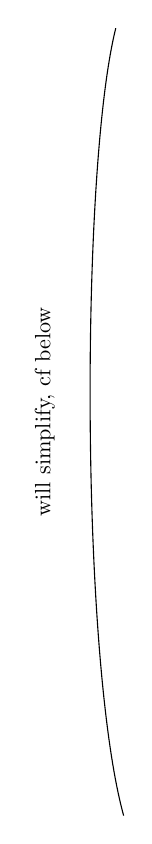
\begin{tikzpicture}[x=1cm,y=1cm]
\draw[line width=.4pt] (1.0,0) .. controls (.45,2.0) and (.45,8.2) .. (.90,10);
\node[rotate=90,anchor=west,scale=.8] at (0,3.7) {will simplify, cf below};
\end{tikzpicture}}}

% @ upper middle, 2°)
2°) $F'\setminus G'\subset F\setminus G$ Let $A'\in F'\setminus G'$, let us prove $A'\in F\setminus G$, and first $A'\in F$. \deleted{\unsure{We have}} Let $A$ be the least element of $F^{A'}$ hence $\underline{\rule[-.15ex]{.35pt}{.55ex}\,A'\unsure{\subset|\in|\subseteq} A^{\unsure{\deleted{\unsure{\prime|\ast|?}}|\varphi|q}},\ A'^{\circ(F')}\subset A^{\unsure{\deleted{\unsure{\prime|\ast|?}}|\varphi|q}\circ(\unsure{F}}\,\rule[-.15ex]{.35pt}{.55ex}}$ let us prove that $A'=A$ (whence $A\in F$). \deleted{\unsure{We have|Now}}

% @ middle, I say
I say that $A\in F\setminus G$ i.e. $A\notin G$, otherwise we would have $A\subset|G|=|G'|$ hence $A'\in G'$ since $A'\in F'$ and $G'\leq F'$, absurd. \deleted{But} Thus $A\in F\setminus G$, hence $A\in F'$, \deleted{and} It follows that $A^{\circ(F)}=A^{\circ(F')}$ (for $F'\preceq F$\inserted{$F'\ll F$ would suffice}\deleted{)} cf lemma below) and \unsure{\uline{indeed}|\deleted{indeed}} \deleted{$\unsure{F|\in|E}$} $A,A'\in F'$ such that $A'^{\circ(F')}\subset A^{\circ(F')}$, which proves $A=A'$.

% @ lower middle, Thus
Thus \unsure{we have} proved that $\deleted{\unsure{F|A}}A'\in F'\setminus G'\Rightarrow A'\in F$. Let us prove that we have $A'\notin G$ (whence $A'\in F\setminus G$\deleted{)}, qed). \unsure{Otherwise|If} we would have $A'\in G$, we would have $A'\subset |G|=|G'|$, whence (as $A'\in F'$ and $G'\leq F'$) $A'\in G'$, absurd.

% @ lower third, cancelled b) to c)
\deleted{b) $\Rightarrow$ c) \inserted{We assume b) i.e. $\varphi$ induces $F'\setminus G'\overset{\sim}{\longrightarrow}F\setminus G$} Let $A\in F\setminus G$, let us prove that $A^{\circ(F)}$ is a \uline{\unsure{str.$^{t}$-open|str.t-open|open stratum} for \deleted{$\unsure{F|A|the}$} $F'$}. Let $A'\in F'\setminus G'$ be the unique element \deleted{of} such that $\varphi(A')=A$.}
% The oblique cancelling strokes end above this final line; state remains open.
\unsure{Let us prove $A'^{\circ(F')}=A^{\circ(F)}$.|\deleted{Let us prove $A'^{\circ(F')}=A^{\circ(F)}$.}}

% @ bottom, b to c
b $\Longleftrightarrow$ c \deleted{\unsure{Set}} We have $|F|\setminus|G|=|F'|\setminus|G'|$, say $U$, Set $F\setminus G=I^{\unsure{\ast|k|+|\leftarrow}},\ F'\deleted{\unsure{\times|\setminus}}\unsure{\setminus}G'=I'^{\unsure{\ast|k|+|\leftarrow}}$ (open subsets of the ordered index sets $I$, \deleted{$\unsure{A|\Delta}$} $(=\unsure{F|P})$, $I'(=F')$. We have
